%% Template para dissertação/tese na classe UFBAthesis
%% versão 0.9.2
%% (c) 2005 Paulo G. S. Fonseca
%% (c) 2012 Antonio Terceiro
%% www.dcc.ufba.br/~terceiro/ufbathesis

\documentclass[msc, a4paper, classic, pt]{ufbathesis}
\usepackage[utf8]{inputenc}
\usepackage{graphicx}

\newcounter{example}[section]
\newenvironment{example}[1][]{\refstepcounter{example}\par\medskip
   \noindent \textbf{Exemplo~\theexample. #1} \rmfamily}{\medskip}


%% Preâmbulo:
%% coloque aqui o seu preâmbulo LaTeX, i.e., declaração de pacotes,
%% (re)definições de macros, medidas, etc.

\title{<TÍTULO DA OBRA>}
\date{<DATA DA DEFESA>}
\author{Matheus Cardoso de Andrade Silva}
\adviser{Prof. Dr. Angelo Loula}
\coadviser{Prof. Dr. Matheus Pires}

\begin{document}

% Folha de rosto
\dmccfrontpage{MMCC-Msc-XXXX}
% Se seu trabalho não for uma tese de doutorado do DMCC, apague a linha
% acima e use \frontpage

%%
%% Parte pré-textual
%%
\frontmatter

% Portada (apresentação)
\dmccpresentationpage
% Se seu trabalho não for uma tese de doutorado do DMCC, apague a linha
% acima e use \presenationpage

% Ficha catalográfica
\authorcitationname{<SEU NOME EM CITAÇÕES>} % e.g. Terceiro, Antonio Soares de Azevedo
\advisercitationname{<NOME DO SEU ORIENTADOR EM CITAÇÕES>} % e.g. Chavez, Christina von Flach Garcia
\coadvisercitationname{<NOME DO SEU CO-ORIENTADOR EM CITAÇÕES>} % e.g. Mendonca, Manoel Gomes de
\catalogtype{<TIPO DE TRABALHO>} % e.g. ``Tese (doutorado)''
\catalogtopics{<TOPICOS PARA FICHA CATALOGRAFICA>} % e.g. ``1. Complexidade Estrutural. 2. Engenharia de Software''
\catalogcdd{<NUMERO CDD>} % e.g. ``CDD 20.ed. XXX.YY'' (esse número vai lhe ser dado pela biblioteca)
\catalogingsheet

% Termo de aprovação - exemplo
% Modifique com os membros da sua banca
\approvalsheet{Salvador, <DIA> de <MÊS> de <ANO>}{
  \comittemember{Profa. Dra. Professora 1}{Universidade XYZ}
  \comittemember{Prof. Dr. Professor 2}{Universidade 123}
  \comittemember{Profa. Dra. Professora 3}{Universidade ABC}
  \comittemember{Prof. Dr. Professor 4}{Universidade HJKL}
  \comittemember{Profa. Dra. Professora 5}{Universidade QWERTY}
}

% Agradecimentos
% Se preferir, crie um arquivo à parte e o inclua via \include{}
\acknowledgements
<DIGITE OS AGRADECIMENTOS AQUI>

% Resumo em Português
% Se preferir, crie um arquivo à parte e o inclua via \include{}
\resumo
<DIGITE O RESUMO AQUI>
% Palavras-chave do resumo em Português
\begin{keywords}
<DIGITE AS PALAVRAS-CHAVE AQUI>
\end{keywords}

% Resumo em Inglês
% Se preferir, crie um arquivo à parte e o inclua via \include{}
\abstract
% Palavras-chave do resumo em Inglês
\begin{keywords}
<DIGITE AS PALAVRAS-CHAVE AQUI>
\end{keywords}

% Sumário
% Comente para ocultar
\tableofcontents

% Lista de figuras
% Comente para ocultar
\listoffigures

% Lista de tabelas
% Comente para ocultar
\listoftables

%%
%% Parte textual
%%
\mainmatter

% É aconselhável criar cada capítulo em um arquivo à parte, digamos
% "capitulo1.tex", "capitulo2.tex", ... "capituloN.tex" e depois
% incluí-los com:
% \include{capitulo1}
% \include{capitulo2}
% ...
% \include{capituloN}
%
% Importante: Use \xchapter ao invés de \chapter, conforme exemplo abaixo.

\xchapter{Introdução}{}

\begin{itemize}

\item Motivações
\begin{itemize}
\item As opiniões são as principais influenciadoras do comportamento humano (Liu, 2012);
\item Pessoas pedem opiniões a outras pessoas para consumo (mídia, produtos, etc.), posições políticas, religiosas, etc.;
\item Empresas precisam saber as opiniões de seus consumidores;
\item A internet e a web mudaram a forma de comunicação entre pessoas e organizações;
\item Há mais facilidade de acesso a fontes de informações e de disponibilização de opiniões (USAR DADOS PARA EMBASAR ESSA INFORMACAÇÃO);
\end{itemize}

\item Problemas
\begin{itemize}
\item Grande quantidade e diversidade de fontes de opiniões;
\item Diferentes formatos, problemas de sintaxe, gírias, dentro outros;
\item É difícil para uma pessoa comum extrair e resumir opiniões de centenas ou milhares de fontes (USAR EMBASAMENTO);
\item Opiniões são carregadas de sentimentos subjetivos e imprecisos;
\end{itemize}

\item Proposta / Definição
\begin{itemize}
\item É preciso utilizar uma metodologia para lidar com imprecisões e vagueza;
\item Lógica fuzzy (Zadeh, 1965): É uma metodologia da Inteligência Computacional que trata computacionalmente dados imprecisos e vagos;
\item ANGELO: poucos trabalhos sobre a aplicação de lógica fuzzy e/ou sistemas fuzzy foram encontrados, e os encontrados são limitados (tipo de limitação?), demonstrando uma lacuna de pesquisa sobre a aplicação de sistemas fuzzy para mineração de opiniões 
\item Por todos os problemas citadas, associadas as motivações, torna-se evidente a necessidade de sistemas automáticos de mineração de opiniões;
\item Definição de "Opinion Mining";
\item Pela vagueza das opiniões, a Lógica nebulosa pode ser útil para esses sistemas automatizados;
\item PROPOSTA: Propor e avaliar o desempenho de um sistema automatizado de mineração de opiniões baseado na lógica nebulosa;
\item DIFERENCIAL: 
\begin{itemize}
\item Geração de regras fuzzy;
\item Extração e definição de características dos documentos para geração das regras;
\item Apresentação do uso do método de Wang-Mendel no processo de mineração de opinião;
\end{itemize}

\item Perguntas de pesquisa:
\begin{itemize}
\item Como Lógica Nebulosa pode ser utilizada no processo de mineração de opiniões?
\item Quais são os ganhos, caso existam, do uso de lógica nebulosa em mineração de opiniões?
\item ANGELO: mais umas duas questões de pesquisa
\item ANGELO: depois de escrever os resultados e discussão, revisar esta seção 
\end{itemize}

\item Objetivos secundários:
\begin{itemize}
\item Investigar o estado da arte do uso de Lógica Nebulosa em mineração de opiniões;
\item Formalizar o processo de mineração de opiniões e propor uma aplicação da lógica nebulosa;
\item dentificar e compor uma base de dados para avaliação da proposta;
\item Analisar os resultados e compara-los com outros métodos da literatura;
\end{itemize}
\end{itemize}
\end{itemize}

\xchapter{Revisão da literatura}{}

\begin{itemize}
\item A área de mineração de opiniões é recente (Pang and Lee, 2008);
\item Tão recente que ainda existem problemas de terminologias (mineração de opinião, análise de sentimentos, mineração de sentimentos, análise afetiva, dentre outros);
\item Definição de opinion mining (usar um cara forte para isso, como Lib Bing, Po Pang, Turney, etc.)

\item Definição formal de opinião 'O':
\begin{itemize}
\item O = (g, s), onde \emph{g} é o alvo e \emph{s} é o sentimento associados a opinião
\end{itemize}

\item Níveis de mineração de opinião (cita e depois explica cada um deles e diz qual foi usado e por que. Além de, claro, falar de trabalhos que se encaixam em cada nível)
\begin{itemize}
\item Nível de documento;
\item Nível de sentença;
\item Nível de entidades e seus aspectos
\end{itemize}

\item Lógica Fuzzy
\begin{itemize}
\item Muitas das informações que lidamos são imprecisas e vagas;
\item A lógica clássica não consegue lidar com esse tipo de informação;
\item Para isso,Zadeh (1965) propôs a Lógica Nebulosa para lidar com informações vagas e imprecisas

\item Conjuntos Fuzzy
\begin{itemize}
\item A lógica nebulosa diz que um elemento pode fazer parte de mais de um conjunto com graus de pertinência para cada um deles (Uma opinião pode ser positiva e negativa ao mesmo tempo, mas com graus de pertinência para cada conjunto fuzzy)
\item A lógica clássica, por outro lado, determina que um objeto pertençe ou não a um conjunto (Ou uma opinião é positiva ou negativa);
\end{itemize}

\item Wang-Mendel
\begin{itemize}
\item O que é?
\item Explicar o método
\end{itemize}

\item Fala de outros algoritmos de classificação e agrupamento? Tem isso na qualificação, mas não sei se é mais pertinente (??????)

\item Métodos de classificação com uso de regras
\begin{itemize}
\item CFRM
\item GFRM
\end{itemize}
\end{itemize}
\item Trabalhos relacionados
\begin{itemize}
\item Papers with opinion mining? (Angelo: Acho que alguns principais, mais para contextualizar as abordagens, independente e dependente de domínio, classificação com palavras e com features)
\item Papers with both? (angelo: Sim, descrever rapidamente os encontrados e fazer contraste com a nossa proposta)
\end{itemize}

\end{itemize}

\xchapter{Metodologia}{}

O processo de mineração de opinião
\begin{itemize}

\item Preprocessing
\begin{itemize}
\item Definição
\item Reiterar o tipo de análise escolhida: Document Level Analysis
\item Datasets utilizados (Cornell e Amazon - descreve as caracteristicas de cada dataset, como quantidade, balanceamento, natureza, etc.)

\item Descrever e justificar as tarefas envolvidas:
\begin{itemize}
\item O texto é dividido em sentenças
\item POS Tagging - Brill's Tagger
\item Blocos irrealis são filtrados ou não (atualmente NÃO FILTRAM)
\item Defino quais ngrams serão extraídos
\begin{itemize}
\item Defino o uso do tipo de negação (FAR NEGATION - REFER)
\item Os verbos foram recentemente removidos do universo
\item Depois de testar, MANUALMENTE, diferentes configurações de n-grams, mantendo os demais parametros fixos, restaram adjetivos e adverbios, com unigrams, bigrams e trigrams
\end{itemize}

\item Retorna um vetor de n-grams (bag-of-words)
\item Resume o subcapitulo e finaliza falando da saída dessa fase para a próxima
\end{itemize}
\end{itemize}
\end{itemize}

O processo de mineração de opinião é comumente definido em seis etapas: a i) definição do domínio, ii) pré-processamento, iii) transformação, iv) seleção de características, v) classificação e vi) análise dos resultados \cite{moraes2012document}. Cada etapa inclui diferentes tarefas que, dado um documento na entrada do processo, seja possível classifica-lo e avaliar a classificação realizada.

\begin{figure}[h]
\caption{Etapas do processo de mineração de opinião.}
\centering
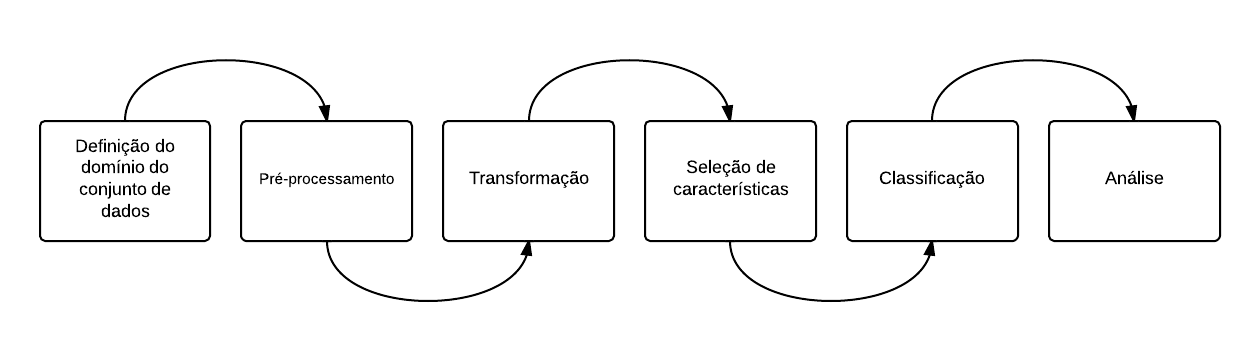
\includegraphics[scale=0.35]{opinion_mining_process.png}
\label{figura:processo_mineracao}
\end{figure}

\section{Definição do domínio e o pré-processamento dos dados}

Domínios diversos foram escolhidos para serem analisados por essa pesquisa, dentre eles filmes, livros, carros, computadores, panelas, hotéis, músicas, celulares, mp3, pen-drives, dispositivos gps, wifi e câmeras fotográficas. Essa diversidade de domínios é importante para que nós possamos corroborar nossa proposta de criar um classificador independente de domínio. Todas as bases de dados são da língua inglesa, pois os trabalhos relacionados a esta pesquisa utilizaram domínios nessa língua.

Para filmes, nós utilizamos a largamente utilizada \footnote{Vide https://www.cs.cornell.edu/people/pabo/movie-review-data/otherexperiments.html} base de dados, versão 2.0, desenvolvida e pré-classificada por \cite{pang2004sentimental}, com 2000 críticas de filmes, sendo metade positivas e outra metade negativas - bases assim, são conhecidas como balanceadas. As opiniões dos domínios de livros, carros, computadores, panelas, hotéis, músicas, celulares estão reunidos numa base de dados balanceada produzida por \cite{taboada2011lexicon}, retiradas do site Epinions \footnote{Vide http://www.epinions.com/}, com cerca de 400 críticas. E para as opiniões dos domínios de mp3, pen-drives, dispositivos gps, wifi e câmeras fotográficas, nós utilizamos uma base de dados balanceada de 2000 críticas retiradas do site da Amazon. 

Após a definição de um ou mais domínios é preciso, antes de inciar a etapa de pré-processamento, definir o nível da análise que será feita sobre os documentos. Existem três níveis básicos de análise de documentos em mineração de opinião: i) nível de análise de documento, ii) sentenças e iii) entidades e seus aspectos. O primeiro nível foca em classificar a opinião geral de um documento expressando-a como positiva ou negativa. O segundo nível, o de sentenças, em vez de considerar o sentimento geral das opiniões presentes em um documento como todo, classifica as opiniões de cada sentença separadamente. E o último nível foca em descobrir todos os alvos existentes nas sentenças do documento, e classifica as opiniões direcionadas a eles \cite{bing:2012}. Este trabalho decidiu utilizar o nível de análise de documento \cite{joachims1998text, pang2002thumbs, gamon2004sentiment, mullen2004sentiment, pang2004sentimental, cui2006comparative}.

A etapa de pré-processamento envolve tarefas como a tokenização dos documentos, marcação gramatical das palavras (do inglês, \textit{Part of Speech Tagging} ou POST), filtragem de sentenças com modais e definição os n-grams que serão utilizados para construir um modelo que represente o documento. A tokenização dos documentos é a tarefa que divide o conteúdo de cada documento em sentenças e, por sua vez, em palavras para que o marcador gramatical (ou \textit{tagger}) possa identificar as classes gramaticais das palavras do documento. O marcador gramatical usado foi o discutido em \cite{brill1995transformation} e usado em trabalhos relacionados a esta pesquisa \cite{chaovalit2005movie, taboada2008extracting, taboada2011lexicon}. A tarefa seguinte é a remoção de sentenças que possuem verbos modais. Segundo \cite{taboada2011lexicon}, modais como "would", "could", dentre outros, presentes numa sentença indicam que as palavras que aparecem juntamente com eles podem não ser confiáveis para serem usadas na definição do sentimento geral de opiniões de um documento. 

A tarefa final é definir quais n-grams serão usados para compor o modelo que representará o documento. O tipo de modelo utilizado nessa pesquisa é o popular saco de palavras (\textit{bag-of-words}), onde cada documento é representado por um vetor de termos (ou n-grams) do documento \cite{moraes2012document}. N-grams são termos que podem ser unigrams (uma palavra), bigrams (duas palavras) ou trigrams (três palavras). Nós definimos 5 tipos de n-grams: adjetivos e advérbios como unigrams; advérbios com adjetivos (e.g. \textit{very good}), advérbios com advérbios como bigrams; e a combinação de dois advérbios e um adjetivo como trigram (e.g. \textit{not very nice}) \cite{pang2002thumbs, turney2002thumbs, taboada2008extracting, karamibekr2012verb}. Nós também extraímos tipos especiais de bigrams e trigrams que são os n-grams negados (e.g. \textit{not bad}, \textit{nothing special}). A extração desses tipos de n-grams também é conhecido com detecção de negação e, por si só, é um linha de pesquisa completa, indo além do escopo deste trabalho. Nós utilizamos uma versão simplificada da técnica usada em \cite{taboada2011lexicon}. 

Ao fim do estágio de pré-processamento, cada documento é transformado num vetor de saco de palavras e é passado para a etapa de transformação. 

\section{Transformação}

\section{Seleção de características}

\section{Classificação}

\section{Avaliação}

\section{Design dos experimentos}

\xchapter{Resultados obtidos}{}

\xchapter{Considerações finais e trabalhos futuros}{}

\backmatter

% Apêndices
% Comente se não houver apêndices
\appendix
%\xchapter{Apêndices}{}
% É aconselhável criar cada apêndice em um arquivo à parte, digamos
% "apendice1.tex", "apendice.tex", ... "apendiceM.tex" e depois
% incluí-los com:
\section{Características extraídas dos documentos} \label{sec:appendix1}

\begin{itemize}
\item Características de contagem %20
\begin{itemize}
\item Contagem dos adjetivos positivos
\item Contagem dos adjetivos negativos
\item Contagem dos advérbios positivos
\item Contagem dos advérbios negativos
\item Diferença entre a contagem de adjetivos positivos e negativos
\item Diferença entre a contagem de advérbios positivos e negativos
\item Contagem de adjetivos e bigrams positivos compostos por advérbio e adjetivo
\item Contagem de adjetivos e bigrams negativos compostos por advérbio e adjetivo
\item Contagem de advérbios e bigrams positivos compostos somente por advérbios
\item Contagem de advérbios e bigrams negativos compostos somente por advérbios
\item Contagem dos unigrams e bigrams positivos
\item Contagem dos unigrams e bigrams negativos
\item Contagem de unigrams, bigrams e trigrams positivos 
\item Contagem de unigrams, bigrams e trigrams negativos
\item Diferença entre a contagem positiva e negativa de adjetivos e bigrams compostos por advérbio e adjetivo
\item Diferença entre a contagem positiva e negativa de advérbios e bigrams compostos somente por advérbios
\item Diferença entre a contagem positiva e negativa de unigrams e bigrams
\item Diferença entre a contagem positiva e negativa de unigrams, bigrams e trigrams
\item Quantidade de n-grams extraídos do documento
\item Tamanho do documento (contabiliza todos os n-grams existentes no documento)
\end{itemize}

\item Características de soma %31
\begin{itemize}
\item Soma dos adjetivos positivos
\item Soma dos adjetivos negativos
\item Soma dos advérbios positivos
\item Soma dos advérbios negativos
\item Soma normalizada dos adjetivos positivos
\item Soma normalizada dos advérbios positivos
\item Soma normalizada dos adjetivos negativos
\item Soma normalizada dos advérbios negativos
\item Diferença entre a soma dos adjetivos positivos e negativos
\item Diferença entre a soma dos advérbios positivos e negativos
\item Soma dos adjetivos e dos bigrams positivos formados por advérbio e adjetivo
\item Soma dos adjetivos e dos bigrams negativos formados por advérbio e adjetivo
\item Soma dos advérbios e dos bigrams positivos somente formados por advérbios
\item Soma dos advérbios e dos bigrams negativos somente formados por advérbios
\item Soma dos unigrams e bigrams positivos
\item Soma dos unigrams e bigrams negativos
\item Soma dos unigrams, bigrams e trigrams positivos
\item Soma dos unigrams, bigrams e trigrams negativos
\item Soma normalizada dos adjetivos e dos bigrams positivos formados por advérbio e adjetivo
\item Soma normalizada dos adjetivos e dos bigrams negativos formados por advérbio e adjetivo
\item Soma normalizada dos advérbios e dos bigrams positivos somente formados por advérbios
\item Soma normalizada dos advérbios e dos bigrams negativos somente formados por advérbios
\item Soma normalizada dos unigrams e bigrams positivos
\item Soma normalizada dos unigrams e bigrams negativos
\item Soma normalizada dos unigrams, bigrams e trigrams positivos
\item Soma normalizada dos unigrams, bigrams e trigrams negativos
\item Diferença entre a soma positiva e negativa dos adjetivos e dos bigrams formados por advérbio e adjetivo
\item Diferença entre a soma positiva e negativa dos advérbios e dos bigrams formados somente por advérbios
\item Diferença entre a soma positiva e negativa dos unigrams e bigrams
\item Diferença entre a soma positiva e negativa dos unigrams, bigrams e trigrams
\item Percentual de n-grams negados
\end{itemize}

\item Características de regra máxima %6
\begin{itemize}
\item Classe da polaridade máxima entre os adjetivos de um documento (1 se o maior valor absoluto entre as polaridades for positivo ou -1 se for negativo)
\item Classe da polaridade máxima entre os advérbios de um documento (1 se o maior valor absoluto entre as polaridades for positivo ou -1 se for negativo)
\item Classe da polaridade máxima entre adjetivos e bigrams formados por advérbio e adjetivo (1 se o maior valor absoluto entre as polaridades for positivo ou -1 se for negativo)
\item Classe da polaridade máxima entre advérbios e bigrams formados somente por advérbios (1 se o maior valor absoluto entre as polaridades for positivo ou -1 se for negativo)
\item Classe da polaridade máxima entre unigrams e bigrams de um documento (1 se o maior valor absoluto entre as polaridades for positivo ou -1 se for negativo)
\item Classe da polaridade máxima entre unigrams, bigrams e trigrams de um documento (1 se o maior valor absoluto entre as polaridades for positivo ou -1 se for negativo)
\end{itemize}
\end{itemize}
% \include{apendice2}
% ...
% \include{apendiceM}


% Bibliografia
% É aconselhável utilizar o BibTeX a partir de um arquivo, digamos "biblio.bib".
% Para ajuda na criação do arquivo .bib e utilização do BibTeX, recorra ao
% BibTeXpress em www.cin.ufpe.br/~paguso/bibtexpress
\bibliographystyle{abnt-alf}
\bibliography{../pesquisa}

%% Fim do documento
\end{document}